\section{Evaluation}
\label{sect:experiment} 

\subsection{Experiment Setup}
We evaluated QoSManager on a desktop PC with Intel(R) Core(TM) i7-2600 CPU @ 3.40GHz and 8GB RAM. We used Mininet~\cite{mininet} with Open vSwitch~\cite{openvswitch} to emulate
different network scenarios. Mininet uses OS features to instantiate lightweight virtualization of network hosts and interconnects them with virtual switches, according to a
specified topology configuration. Open vSwitch is a software implementation of a virtual multilayer network switch. QoSManager was implemented on top of Ryu~\cite{ryu}, an
open-source SDN controller.

\reffig{setup} shows our experiment setup. There are two switches connected with a 8Mbps link.

\begin{figure}[htb]
\centering
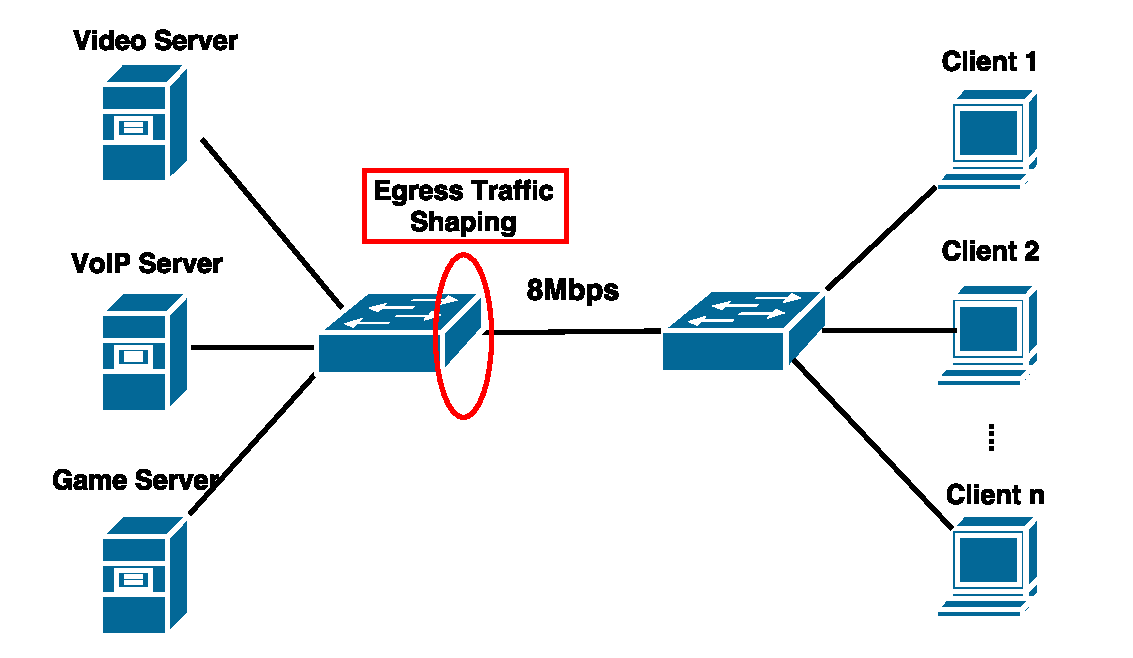
\includegraphics[width=0.5\textwidth]{exp_setup}
\caption{Experiment setup.}
\label{fig:setup}
\end{figure}

During the experiments, different types of services, such as game, video and VoIP, sends traffic to the applications on the right. All the traffic flows through the link between
the two switches and competes for the scarce bandwidth. The Qos requirements for the services are displayed in~\reftable{qos_config}.

\begin{table}[htb]
\scriptsize
\caption{Qos Configuration}
\begin{tabular}{|l|l|l|l|}
\hline Service type & Minimum bw & Recommended bw & Priority \\
\hline
\hline VoIP & 400Kbps & 1.2Mbps & 10 \\
\hline Video & 2.5Mbps & 5Mbps & 8  \\
\hline Game & 1.5Mbps & 3Mbps & 6  \\
\hline
\end{tabular}
\label{table:qos_config}
\end{table}

We first investigate how QoSManager allocates bandwidth to high priority traffic and low priority traffic. Then, we study whether high priority traffic will be affected by
new low priority flow coming into the network. Finally, we analyze whether high priority traffic can achieve the desired bandwidth fast in a congested network.

\subsection{Question1: How does QoSManager allocate bandwidth?}
In this scenario, two hosts are watching videos and one host is making a VoIP call.
The video data is sending to the hosts at rate of 5Mbps, and the VoIP data is sending to the host at rate of 1.2Mbps.
The three hosts are using the network at the same time.  

\reffig{s1_qos} illustrates the bitrates of the three services with our system, and \reffig{s1_no_qos} shows the bitrates of the three services without our system. 

\begin{figure}[htb]
\centering
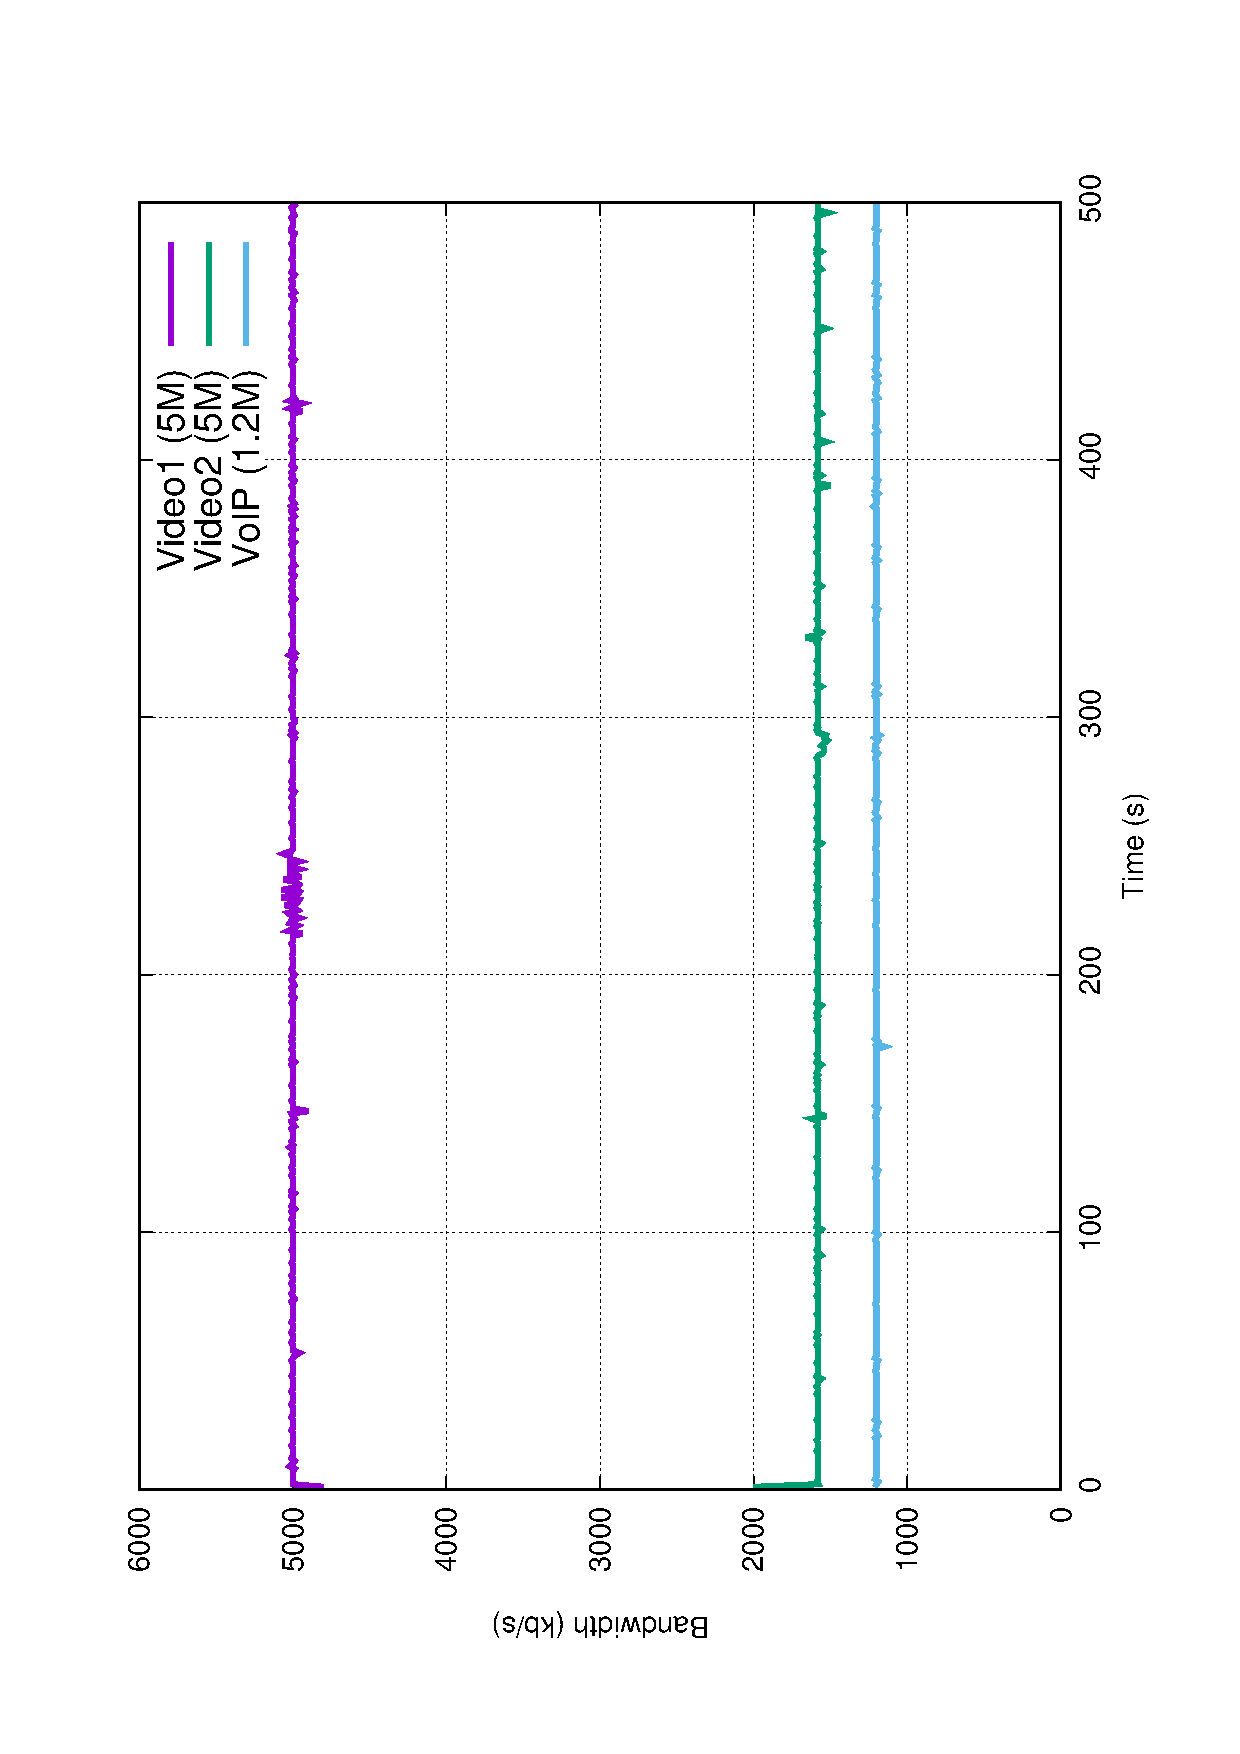
\includegraphics[width=0.32\textwidth,angle=270]{s1_qos}
\caption{Bitrates of services in scenario1 with QoS.}
\label{fig:s1_qos}
\end{figure}


\begin{figure}[htb]
\centering
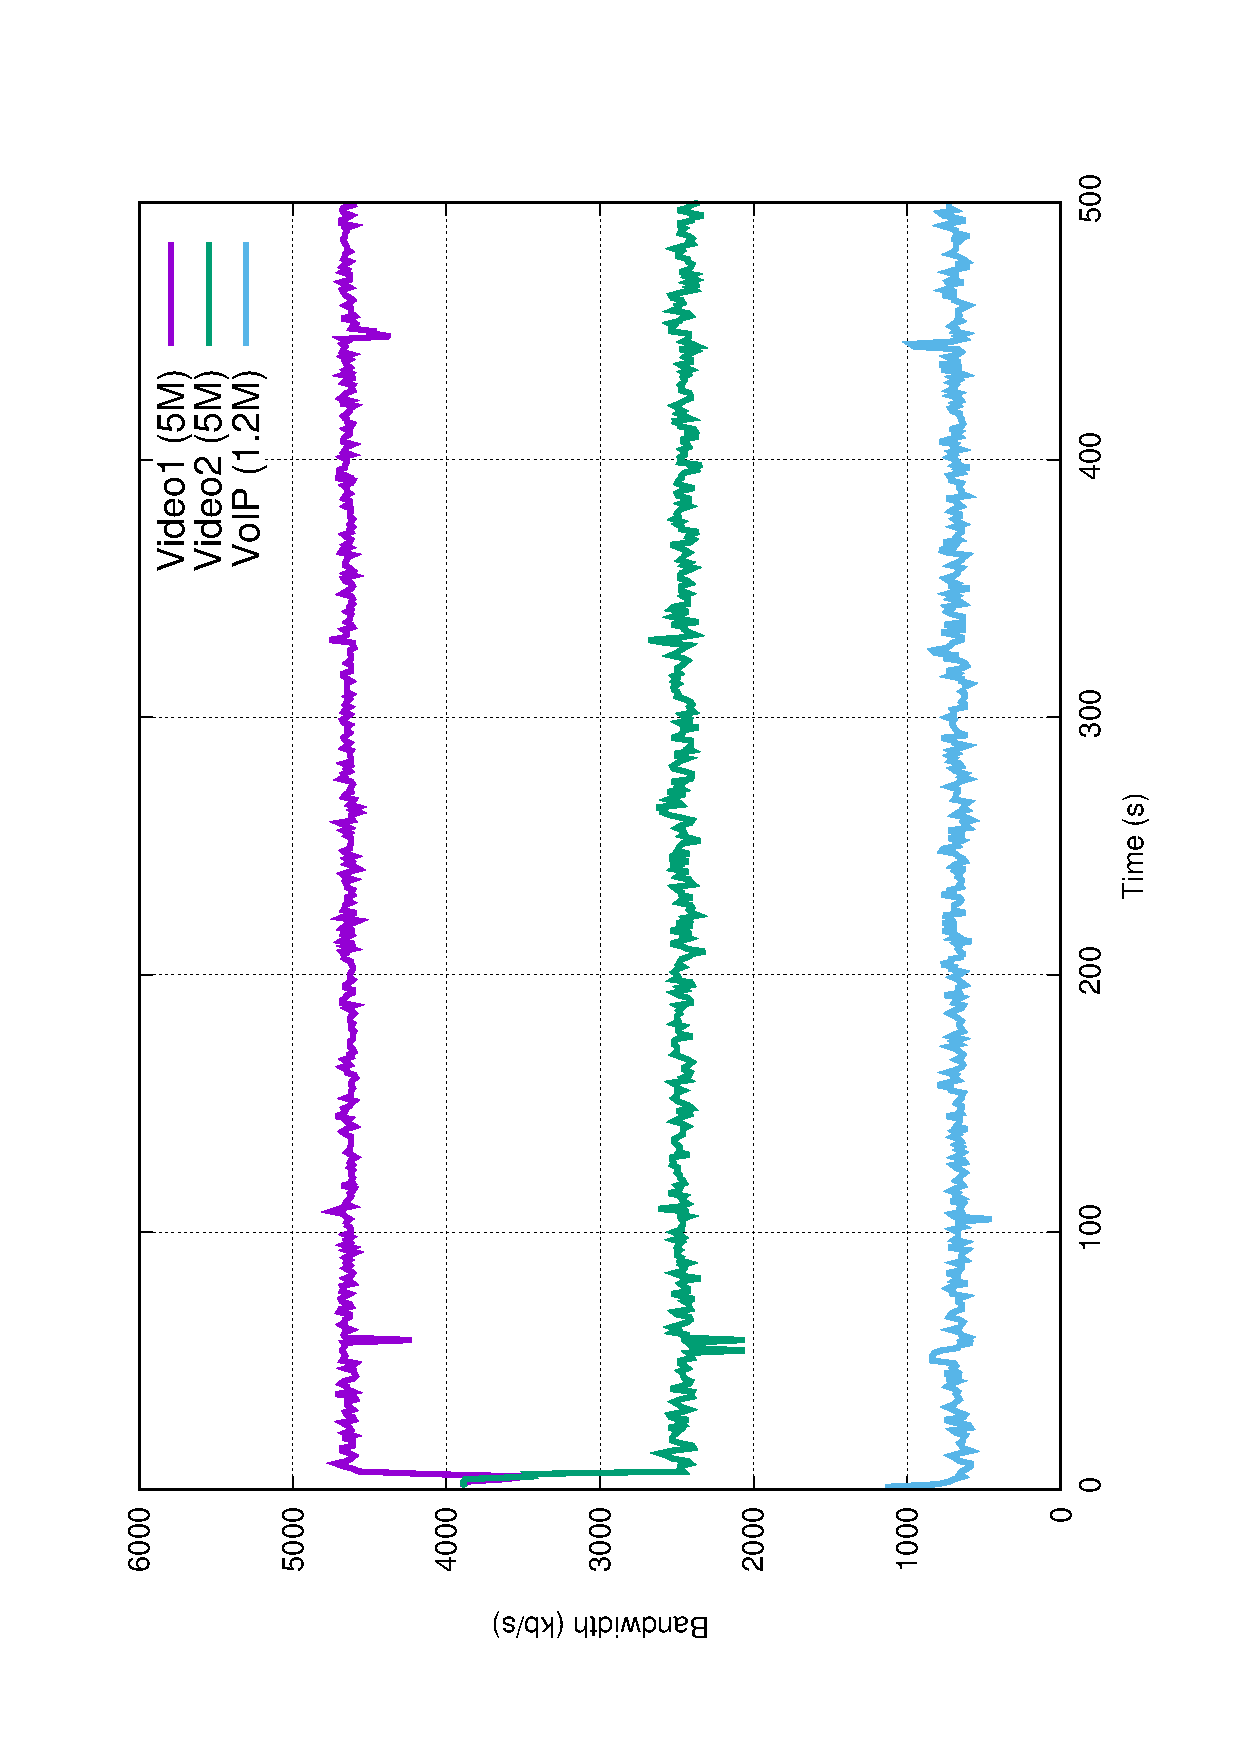
\includegraphics[width=0.32\textwidth,angle=270]{s1_no_qos}
\caption{Bitrates of services in scenario1 without QoS.}
\label{fig:s1_no_qos}
\end{figure}

The results show that our system provides recommended bandwidth for the VoIP flow as VoIP has higher priority than Video. 
Our system also provides recommended bandwidth for one of the video flow. While without QoS, none of three services achieve recommended bandwidth.

\begin{figure}[htb]
\centering
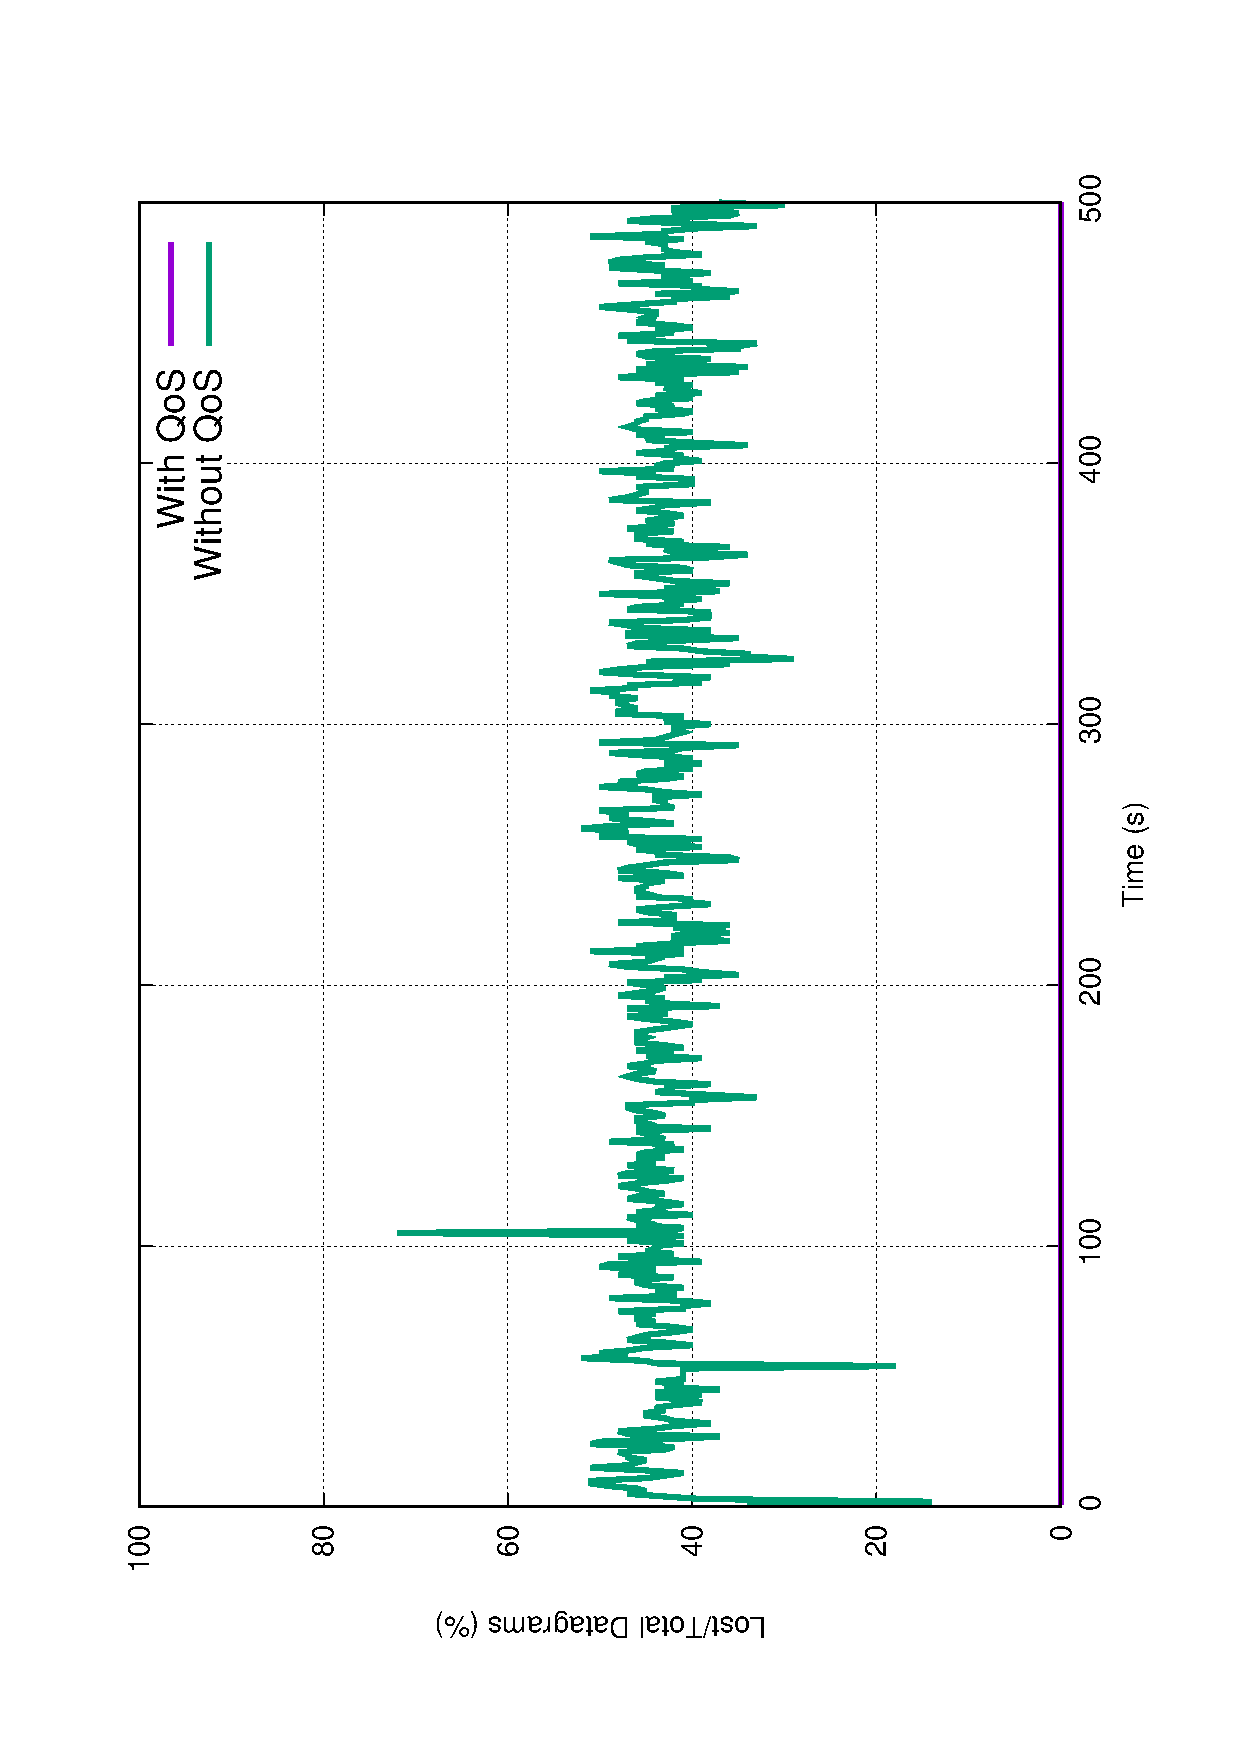
\includegraphics[width=0.35\textwidth,angle=270]{s1_loss}
\caption{Comparison of packets loss for VoIP with and without QoS.}
\label{fig:s1_loss}
\end{figure}

\reffig{s1_loss} shows the packet loss rate for the VoIP flow with and without QoS. As our system provides recommended bandwidth for VoIP, there is no packet loss. Without QoS, the packet loss rate is about 50 percent. Our system greatly improves the quality of VoIP call when there is competing network.

Thus, our system improves QoS of user perferred services and also reduces bitrate oscillation. 

\subsection{Question 2: How is high priority traffic affected by low priority traffic?}
In this scenario, one host starts watching video which lasts 500s. After 50s, another host starts play a game which lasts 400s. After another 50s, another host starts another game which lasts 300s.
The video data is sending to the host at rate of 5Mbps, and the game data is sending to the hosts at rate of 3Mbps.

\begin{figure}[htb]
\centering
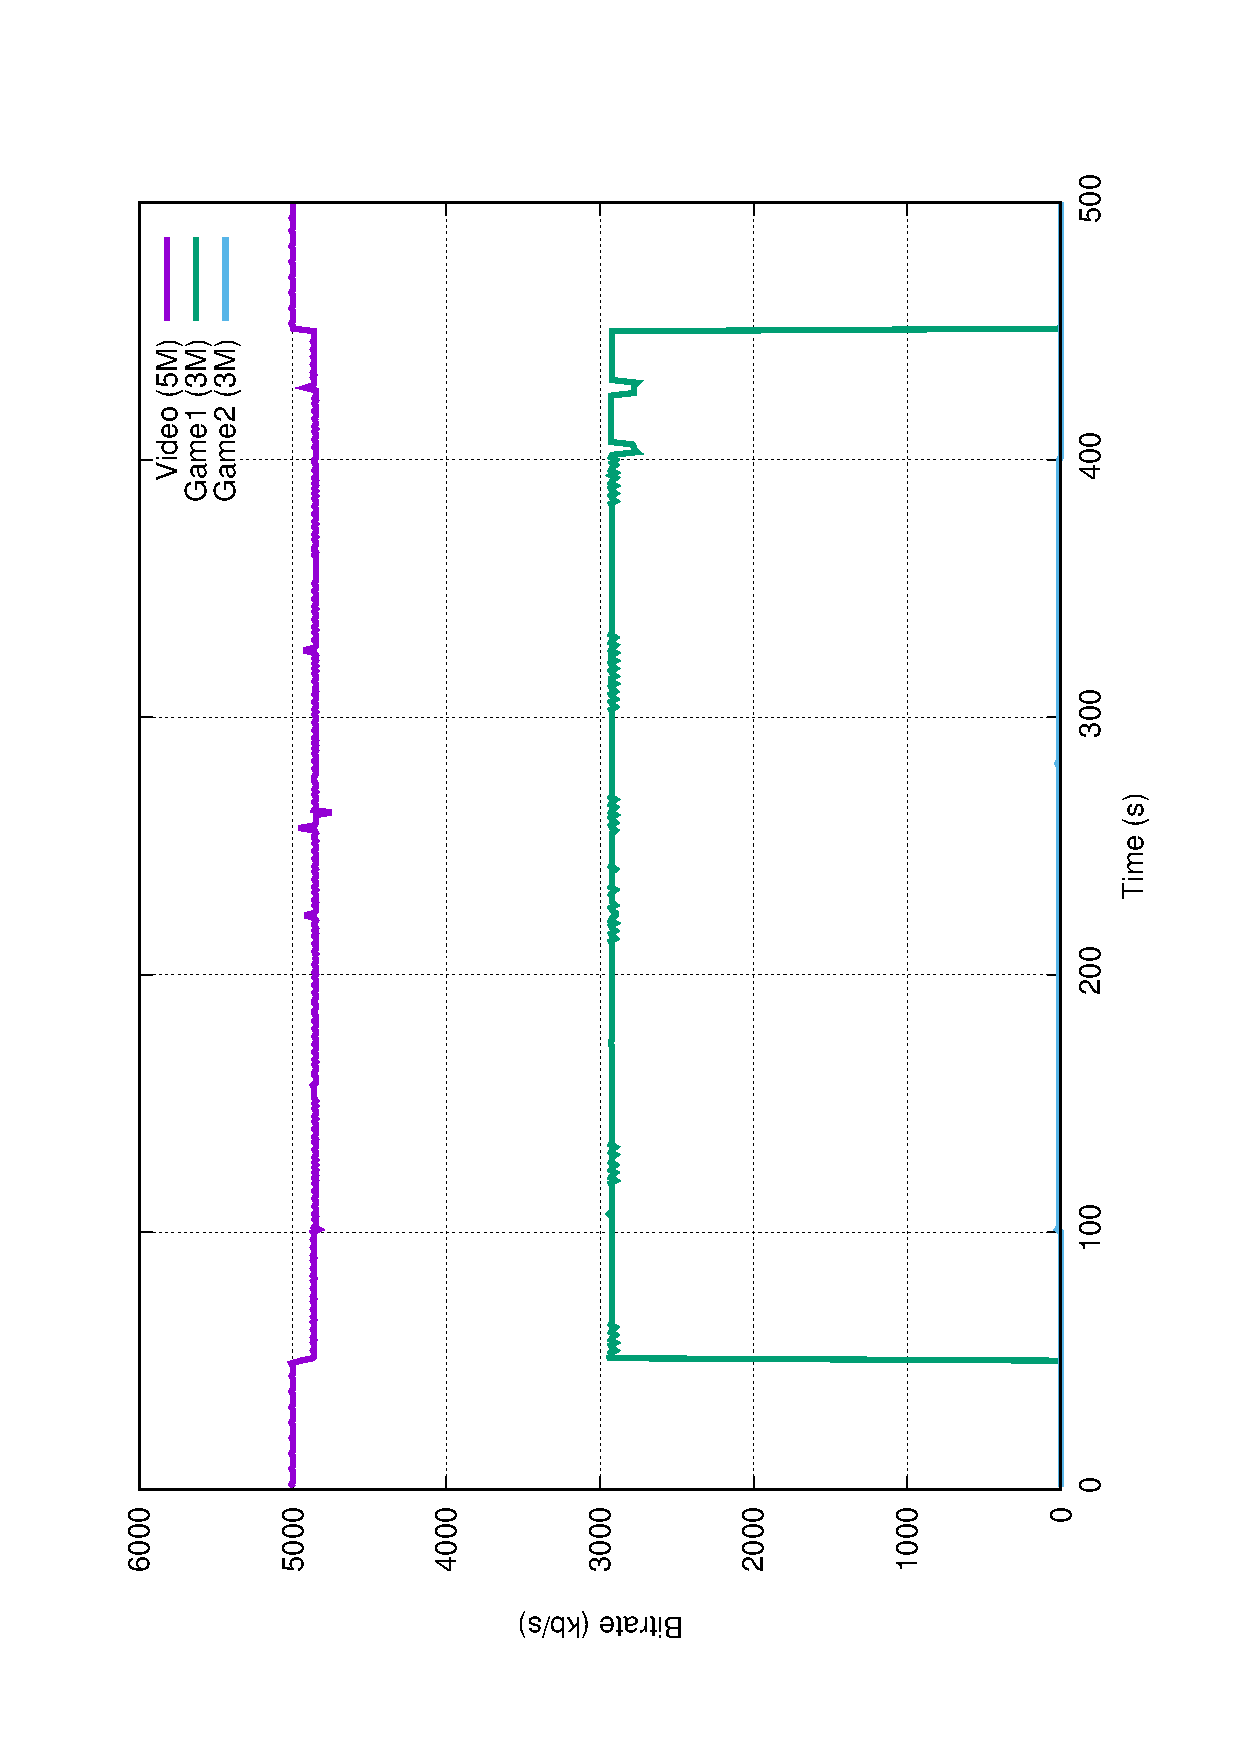
\includegraphics[width=0.32\textwidth,angle=270]{s2_qos}
\caption{Bitrates of services in scenario2 with QoS.}
\label{fig:s2_qos}
\end{figure}

\begin{figure}[htb]
\centering
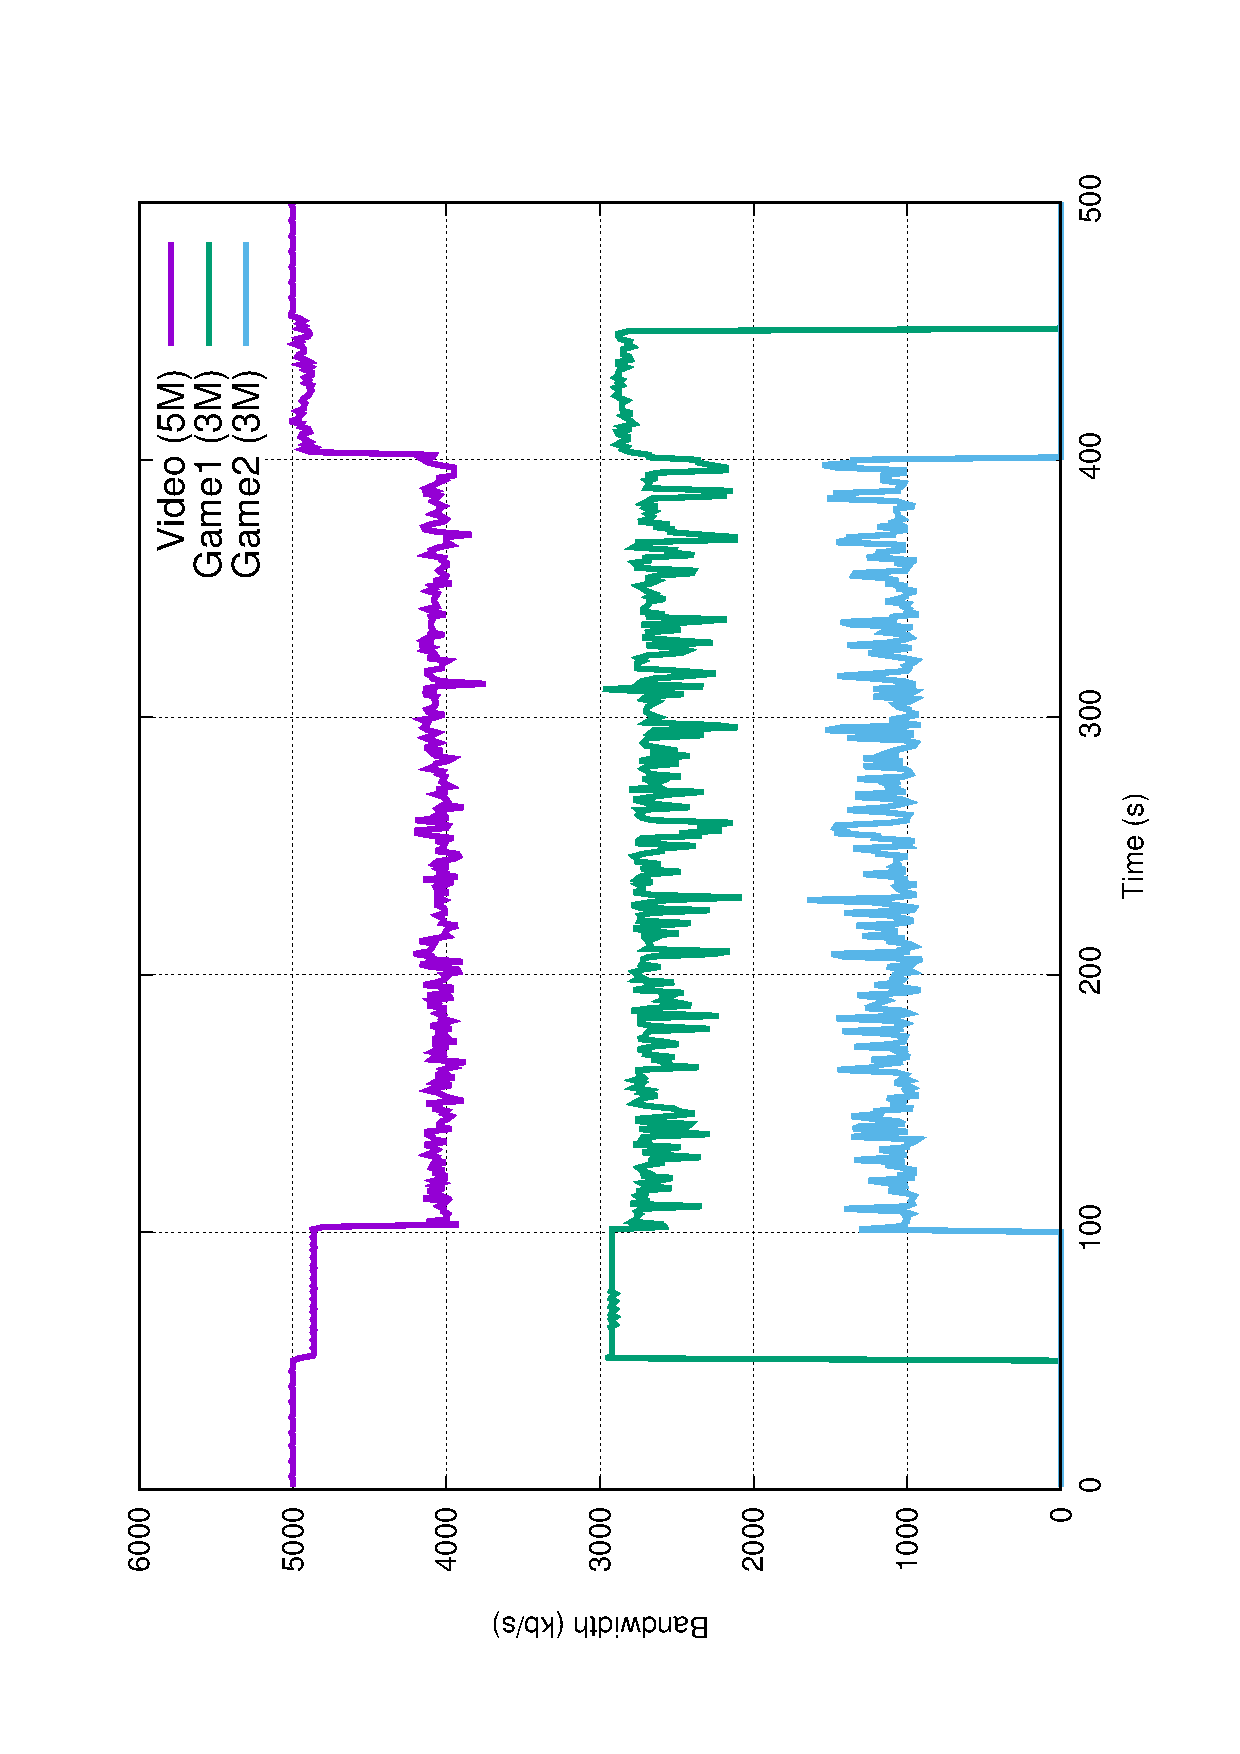
\includegraphics[width=0.32\textwidth,angle=270]{s2_no_qos}
\caption{Bitrates of services in scenario2 without QoS.}
\label{fig:s2_no_qos}
\end{figure}

\reffig{s2_qos} illustrates the bitrates of the three services with our system, and \reffig{s2_no_qos} shows the bitrates of the three services without our system. 
With our system, as the priority of video is higher than game. The bandwidth of vidoe is not affected by the incomming game flows. Our system also provides recommended bandwidth for the first joined game flow.
Without QoS, the bandwidth of both the video and the first joined game is reduced when the second game flow comes. Also, none of the three services acheive recommended bandwidth.

Thus, in our system, services with higher priority will not be affected by services with lower priority.

\subsubsection{Scenario 3}
In this scenario, two hosts are play games. After 50s, another host starts watching a video which lasts 400s. After another 50s, another host starts making a VoIP call which lasts 300s.

\begin{figure}[htb]
\centering
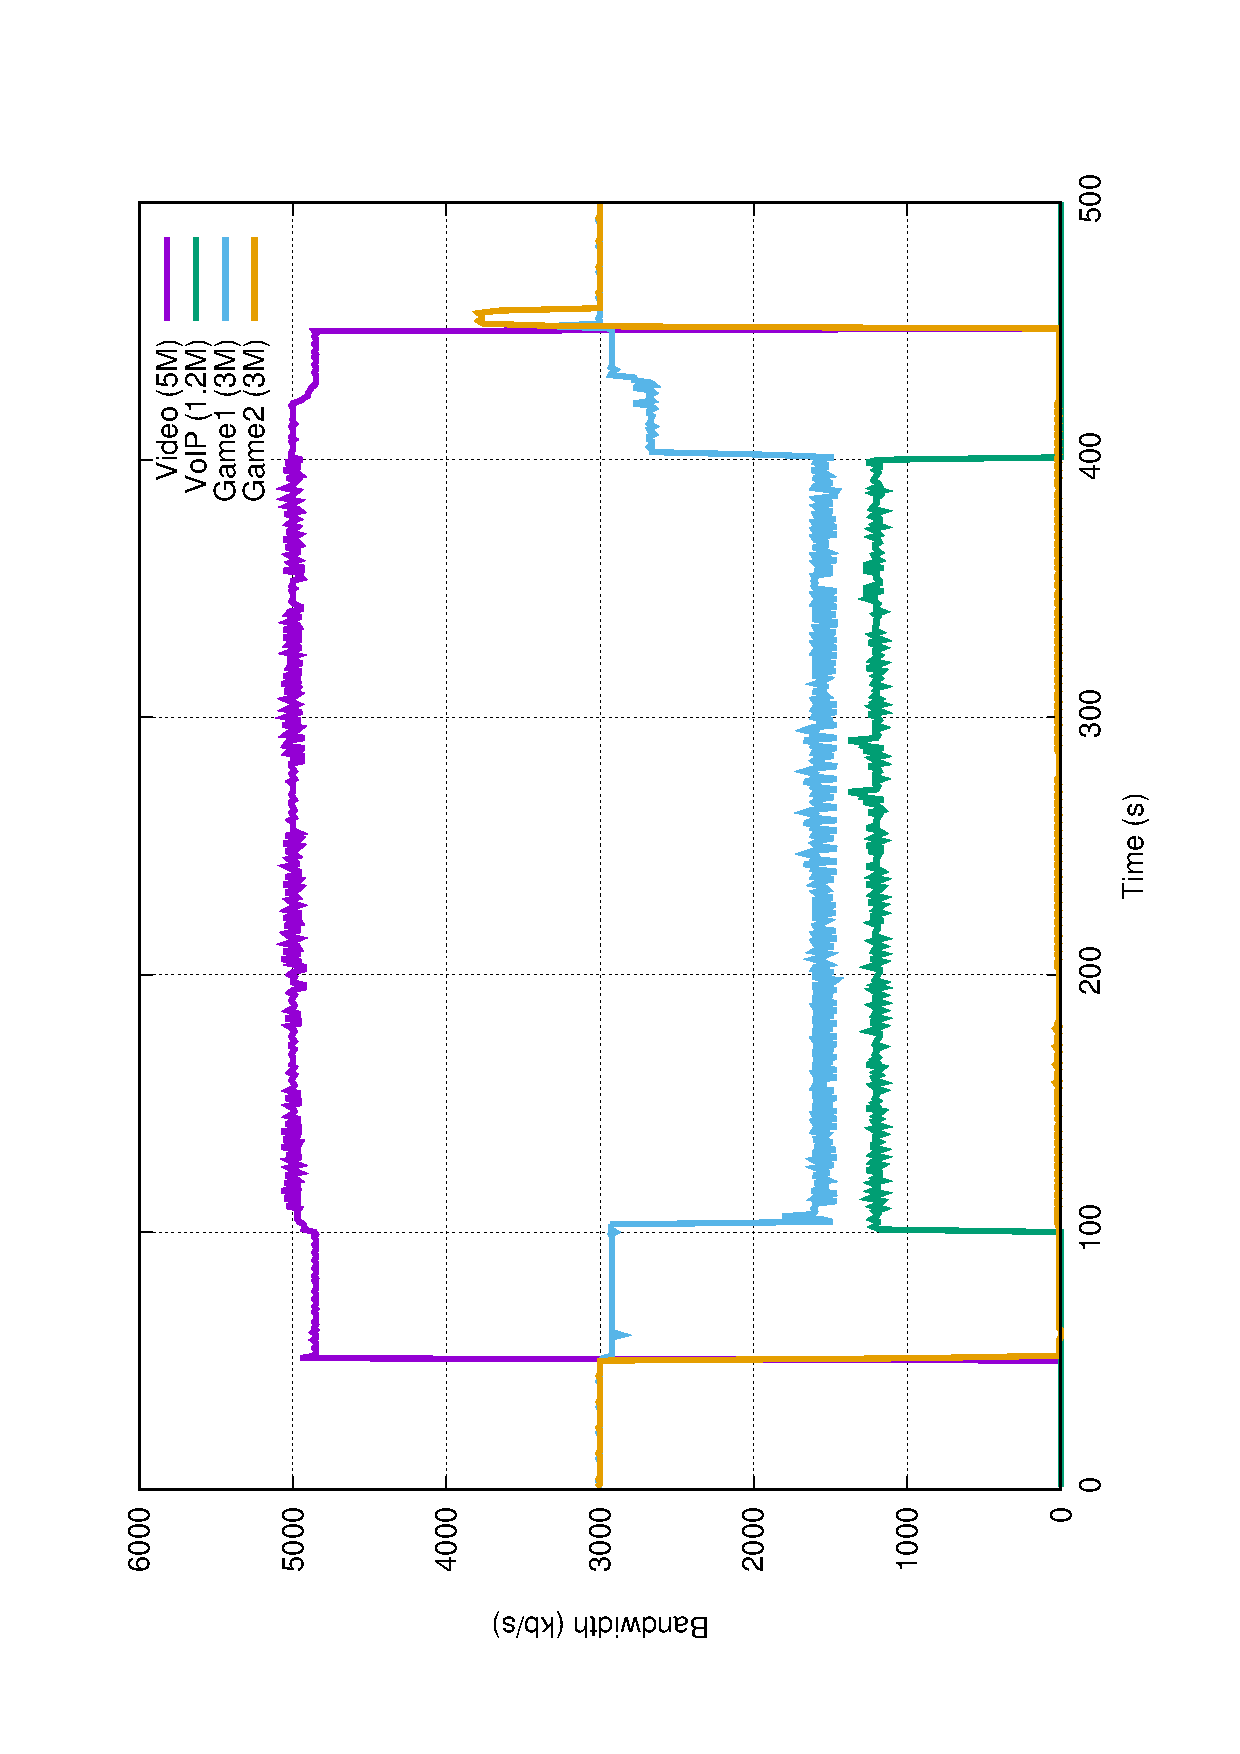
\includegraphics[width=0.35\textwidth,angle=270]{s3_qos}
\caption{Bitrates of services in scenario3 with QoS.}
\label{fig:s3_qos}
\end{figure}

\begin{figure}[htb]
\centering
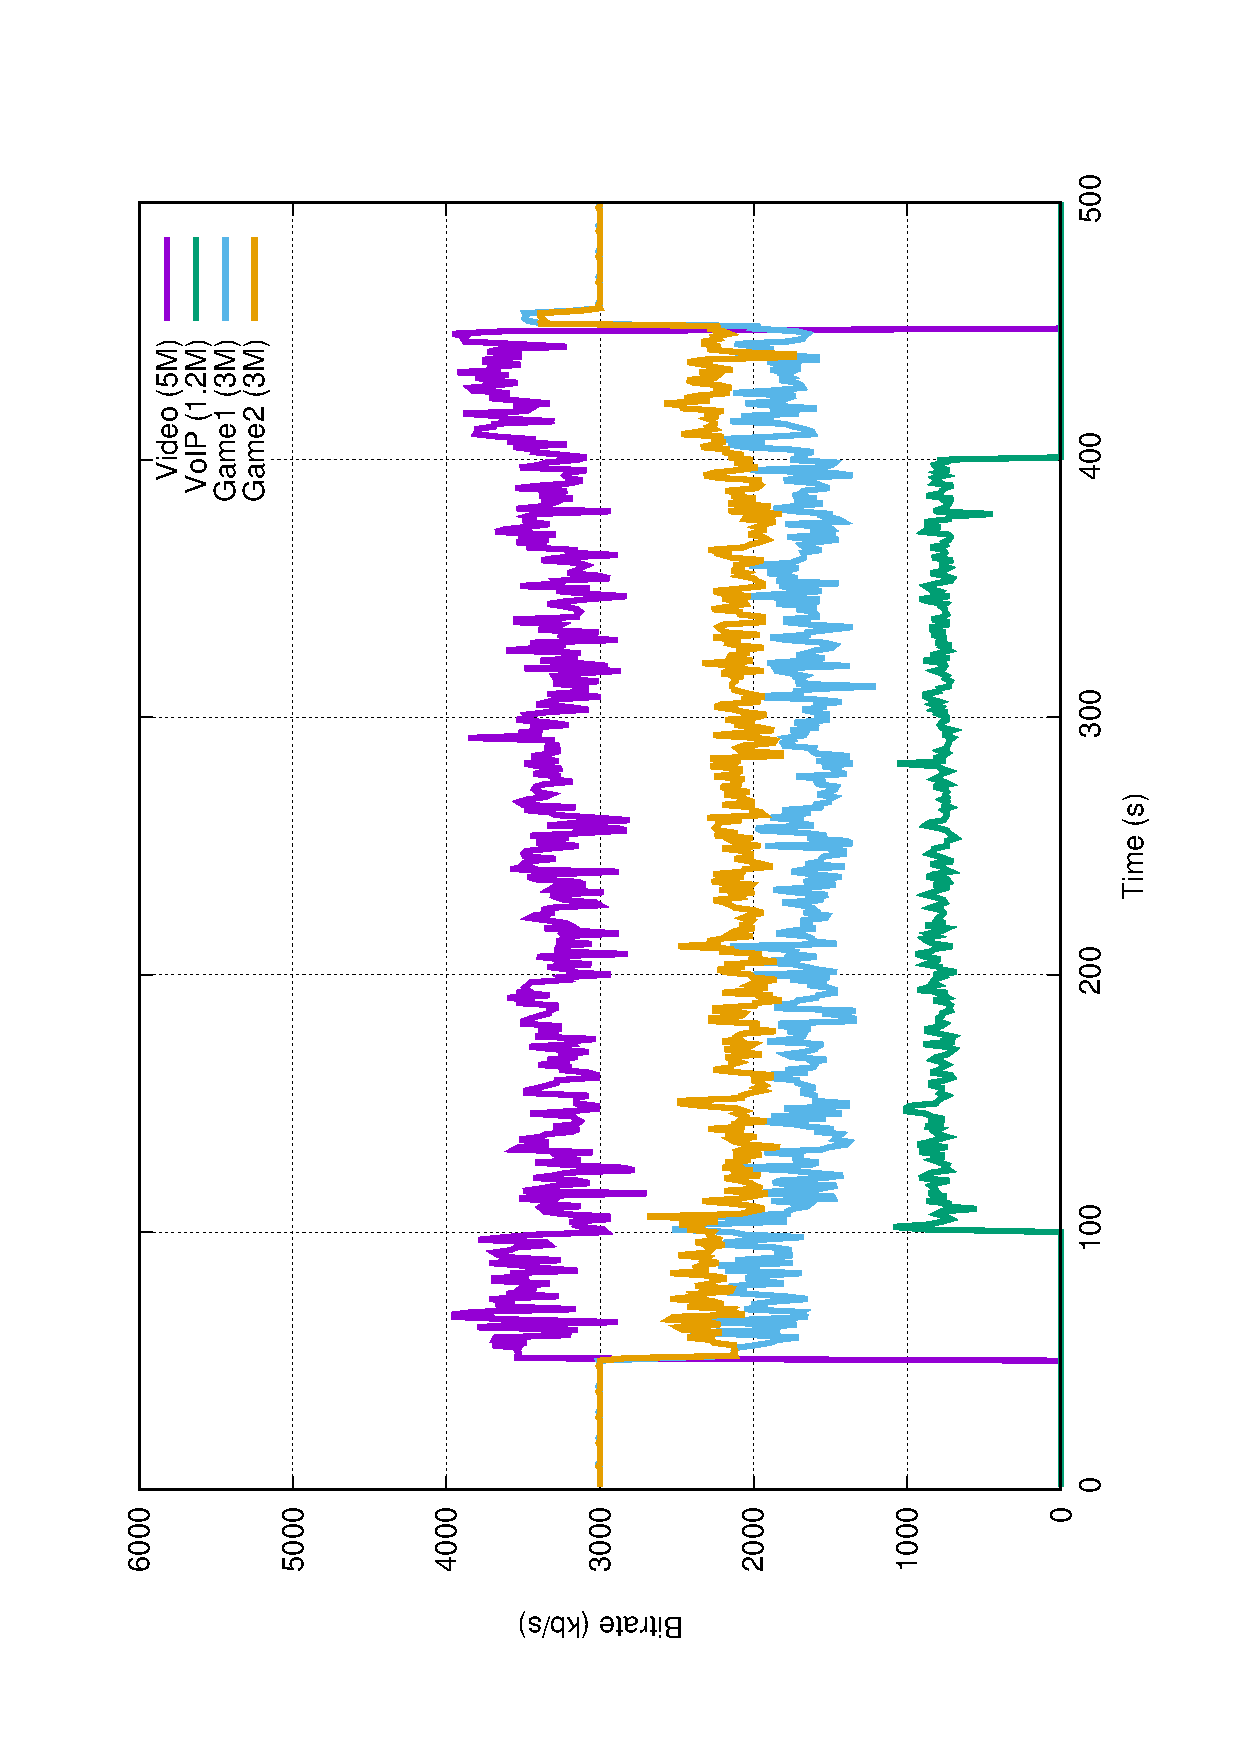
\includegraphics[width=0.35\textwidth,angle=270]{s3_no_qos}
\caption{Bitrates of services in scenario3 without QoS.}
\label{fig:s3_no_qos}
\end{figure}

\reffig{s3_qos} illustrates the bitrates of the four services with our system, and \reffig{s3_no_qos} shows the bitrates of the four services without our system. 
With our system, when the video flow comes in, as the priority of video is higher than game, our system reduces bandwidth of one game and provides reommended bandwidth for the video. When the VoIP flow comes in, our system again sacrifices the bandwidth of the other game to provide recommended bandwidth for VoIP as VoIP has the highest priority. When the VoIP flow ends, our system dynamically adjust bandwidth allocation, and uses the bandwidth to provide better quality for one the game.
While without QoS, when the video flow comes in, the bandwidth of both the game flows are reduced. When the VoIP flow comes in, all the bandwidth of video and games are reduced. None of the services has ever achieved recommended bandwidth.

Thus, our system will sacrifice bandwidth of service with lower priority to serve services with higher priority to satisfy the QoS requirements of user.
